\documentclass[xcolor=dvipsnames]{beamer}  %定义文件类型
\usetheme{Copenhagen}                      %此句及以下是我使用的主题和包
\usecolortheme{wolverine}                       %颜色主题
\usepackage{utopia}                             %字体
\usecolortheme[named=brown]{structure}          %改变主题内嵌结构的颜色
\usepackage{CJK}                                %中文包,如果全部英文可以不用

\begin{document}                           %总的开始
\title[幻灯片缩略名]{幻灯片全名}           %以下是幻灯片首页的编辑
\subtitle{副标题}
\author{作者姓名}
\institute{作者所属学校}
\date[\initclock\tdtime]{\today}                     %总是显示当前的日期
\logo{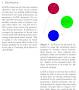
\includegraphics[height=10mm]{1.jpg}} %这是我的logo,如果不需要删掉词句即可
\begin{frame}
	\titlepage
\end{frame}                                %幻灯片首页的编辑到此结束

\begin{frame}                              %开始编辑第i张幻灯片
	
\end{frame}                                %结束编辑第i张幻灯片
\end{document}                             %总的结束
